% 来源：OEBPS/Text/Section0001_split_002.xhtml#sigil_toc_id_17

\BookChapter{8}
\section[第8章\q 投资营销谎言3：“我们的收益——你看到的就是你得到的”]{第8章\\ 投资营销谎言3：“我们的收益——你看到的就是你得到的”}

\begin{BookQuote}
太意外了，基金报告的投资收益并不是投资者真正得到的投资收益。

\hfill ——约翰·博格（先锋公司创始人）
\end{BookQuote}

\begin{BookQuote}
大多数人都很熟悉基金广告里陈词滥调一般的免责声明：历史业绩并不能保证未来业绩。但是极少有人认识到，历史业绩的数据本身会误导投资者。

\hfill ——《基金公司如何合法操纵数据》（《华尔街日报》2013年3月31日）
\end{BookQuote}

\subsection{给猪涂些口红}

2002年，嘉信理财公司投放了一条相当聪明的广告，广告中有个典型的华尔街销售经理，他早上一上班正在他的电话推销办公室里发表演讲，鼓舞士气。“告诉你的客户，这是最火的热门股！热得像烈火！千万别提基本面——很糟糕。”他结束了早上的演讲，挥舞着纽约尼克斯篮球队的场边票，这是奖给那些获胜的销售人员的。他最后大吼一声给大家祝威：“我们来给这头猪涂些口红吧。”

\subsection{只让我看好的那一面}

1954年，达雷尔·哈夫写了本书《统计陷阱》。他指出：“无数的统计数据花招是用来愚弄人的，而不是用来告诉人真实数据的。”今天公募基金行业能够运用一种巧妙的方法计算并公告投资收益，其实就像约翰·博格所说的那样，基金公司报告的投资收益，“并不是投资者真正拿到手的投资收益”。后面我们会解释这种高超的玩弄数字游戏的魔法。在此之前，我们先来弄清楚平均收益的误区。

下面的这张图显示了一种假设的市场行情，它上下波动，就像过山车一样。行情先上涨50\%，再下跌50\%，又上涨50\%，然后又下跌50\%，这样上上下下，结果其平均收益率是0\%。你可能跟我一样会觉得，平均收益率是0\%就意味着我没有亏一分钱。我们都大错特错了！

\begin{figure}[htbp]
\centering
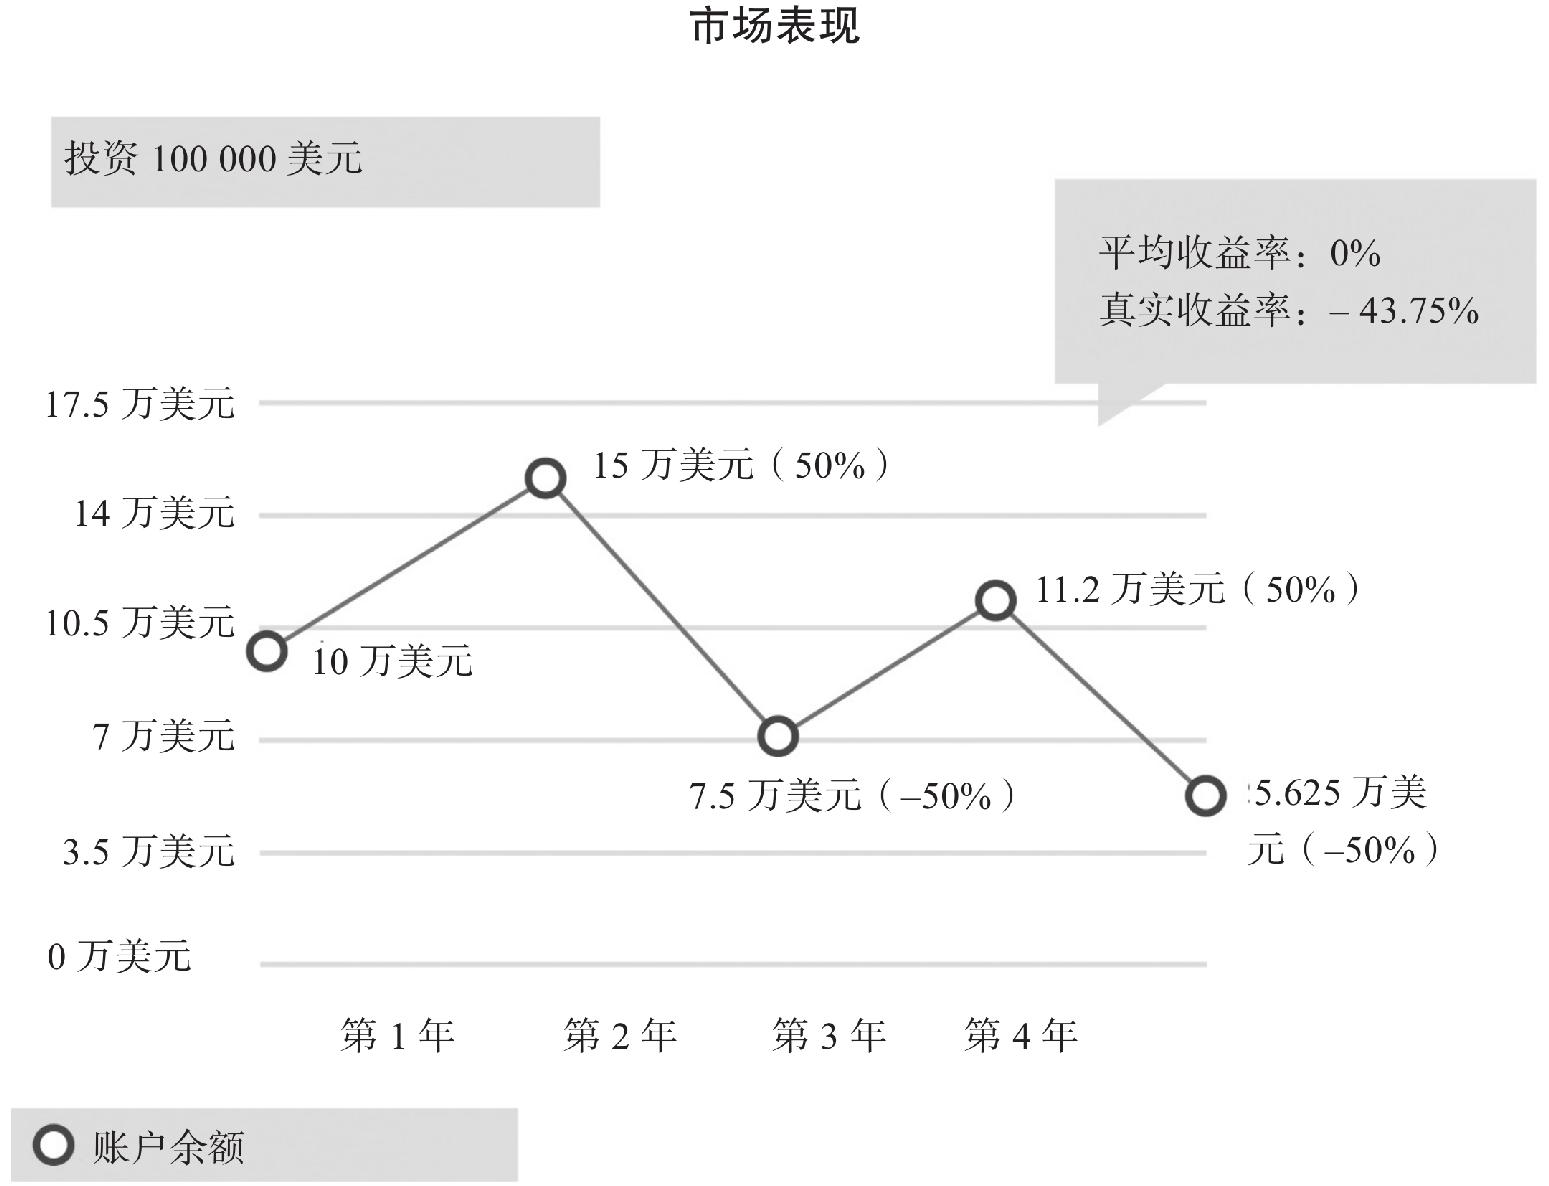
\includegraphics[width=0.82\linewidth,keepaspectratio]{image/8-1.jpg}
\caption{}\label{fig:8-1}
\end{figure}

看看这张图，如果你开始用的是真金白银来做投资，比如你开始用了10万美元，那么到了第4年年底，你实际上亏损了43750美元，亏损比例高达43.75\%！你以为你是盈亏平衡，可是事实上你亏了43.75\%！你事前猜到会是这种结局吗？现在你也是个投资内行了，一定要注意！平均收益率有个内在误区——过于美化投资业绩，但其实这种业绩并不存在。

《福克斯商业》杂志上有篇文章是《解决收益率的迷思》。文章解释了这种不一致如何被运用到真实的世界：“我们可以用另一种方式来看待这种平均收益与实际收益之间的不一致，回顾一下1930年以来的道琼斯指数。我们把过去81年每年的道琼斯指数涨幅加到一起，然后再除以81年，算出来的每年“平均”收益率为6.31\%。可是你自己用复利算一算，就会得到“真实的”年化收益率为4.30\%。为什么这一点非常重要？你在初期，即1930年投资1000美元，如果每年的投资收益率是6.31\%，那么经过81年到现在，你的投资会增值到14.2万美元。如果投资收益率是4.30\%，你的投资只能增值到3万美元。年收益率只相差2.01\%，你81年的投资收益却相差了11.2万美元。

\subsection{收益率要加权计算}

现在我们看到了，平均收益率这个业绩指标并不能真正表明我们赚了多少钱。坐下来放松一下，更大的误区我还没有说呢！华尔街证券投资行业里那些数学魔术师想方设法地来计算他们的投资收益率，好让客户看起来更美好一些。他们是怎么做的？

简而言之，公募基金投放广告宣传自己的具体投资收益率是多少，但正如约翰·博格所说的，这并不是“客户真正赚到手的投资收益率”。为什么？你看在基金公司广告宣传的小册子上看到的投资收益率是时间加权收益率。听起来比较复杂，但其实并不复杂。（不过，别紧张，你肯定一学就会，下次你出去跟别人一起吃饭聚会时，你就可以用这个专业术语了，这会显得你很牛，显得你很懂行。）

公募基金的基金经理说，如果你在这个年度一开始就投资1美元购买这只基金，一直持有到年底，你的基金净值会是1.2美元，你赚了20\%。“发动市场营销部，多搞些整版广告，好好宣传我们这么好的业绩。”但是，事实上投资者很少会在一年刚开始的时候就把所有的钱都投到基金上。投资者一般是一年里陆陆续续地往基金里面投钱——他们一般是每次发工资后就拿出一部分转入401(k)账户，然后再用这些钱去买基金。如果我们是在基金业绩好的时候买更多的基金，而在基金业绩表现比较差的时候少买基金，那么我们实际上得到的投资收益率就和基金广告上宣传的基金业绩差别很大。所以，如果到了年底我们坐下来，把现实情况考虑进去，我们不断地申购基金往基金里面投钱，也不断赎回基金从里面拿钱，我们就会发现自己真正赚了多少钱或者亏了多少钱。这种现实世界真实业绩的计算方式被称为资金加权收益率。资金加权收益率是我们真正拿到手的业绩，而时间加权收益率是基金经理用来做广告吹嘘的业绩。

约翰·博格一直在持续不断地推动改变这种只公告时间加权收益率的行规。他相信投资者应该看到他们到底真正赚了多少钱（或者亏了多少钱），完全根据他们的个人实际操作情况（把申购和赎回都考虑进来）来计算。这听起来就像普通的常识，本来就应该这么做，是不是？但是不足为奇，基金公司都不愿意公告基金投资人的实际业绩。博格说：“我们比较过这两种基金投资业绩，一个是投资者真正赚到手的业绩——资金加权收益率，另一个是基金本身赚到的业绩——时间加权收益率。我们比较之后发现，投资者真正赚到手的业绩要比基金本身的业绩低3个百分点。”噢！如果基金广告上说的业绩是6\%，那么基金投资者实际赚到手的业绩只有3\%左右。

\subsection{真相和解决方案}

平均业绩就像网络约会前你看到对方的资料照片。这些照片都是被美化过的，和他们的真容相比，你会觉得完全是两个人。要想知道开始的时候你的资产净值（基金净值和现金），以及你现在手里的资产净值，那你可以利用网络，输入初期和期末的资产净值，它马上就会算出这段时期你的资金实际取得的收益率到底是多少。

你必须记住，公募基金报告的基金业绩（年化投资收益率）是基于一个理论假设，这个人每年都是在1月1日把所有的钱投进来，并一直持有到当年年底12月31日。这种假设对于大多数人来说是不现实的，所以我们不要误导自己相信基金宣传手册上那些看起来非常亮丽的业绩，就是我们这些基金投资人实际得到的业绩。

\subsection{前路从此不再迷茫}

从来没有人说，爬上一座高山是很容易的。不过如果你有一把大砍刀叫作“真实”，用来砍掉那些谎言，让你前面的道路清晰可见，你的登山之旅就会容易得多。成为一个投资内行，从此以后你就不再是乱飞乱撞的无头苍蝇了。

你现在知道了兜售选股能力公司的基金，在一段持续较长的期限里，并不能战胜市场（特别是你的基金账户在扣除费用和税收之后的净投资收益率会更低）。

你也知道了费用并不是无关紧要的，而是至关重要的。降低你的费用，你就可以拿回你未来潜在投资收益的六成到七成。那么这个令人震惊的真相会对你的未来退休生活产生多么巨大的影响呢？

最后，你还知道了平均收益并没有描绘出真实的收益情况。你实实在在拿到手的收益才是最重要的。现在你有了简单的工具，可以计算出你真正实现的投资收益率。

现在你通向财务自由的旅程远远不只是刚刚起步了。你已经跨出了一大步。你现在所了解到的那些真相，可以让你鹤立鸡群。你再也不是那些盲目投资、任人宰割的羊群中的一只小绵羊了。

\subsection{单飞}

我教过很多人学习掌握这些工具。这些人因此经常感觉他们再也不能相信任何人了。从某种意义上讲，他们觉得自己被那些券商经纪人和银行理财经理出卖了，他们从此真正觉悟了，开始明白投资游戏的真正规则。他们认为现在必须自己亲自动手处理每一件事情，结果让自己变成了一座孤岛，因为“没有人可以信任”。这并不是完全真实的，还有很多非常棒的金融投资专家，他们正直可靠，完全值得信赖，并全心全意地为客户的未来着想。我就有一个非常了不起的投资顾问，我毫无保留地信任他，他会根据我的最佳利益采取行动，我们一起评估和管理我的个人投资。和你一样，我也忙得不可开交，根本没有时间，或者根本不想花时间去管理我的投资组合。实际上，如果正确操作的话，只需要每个季度或者每半年简单评估一次投资组合就足够了。你需要做的就是回顾一下你的投资目标，并对投资组合进行再平衡。

那么你怎么知道你对面的销售人员是只想从你身上赚到最多佣金，还是一个值得信任的投资顾问，可以完全托付你的未来？你又怎么能知道他到底是一个经纪人，还是一个投资向导？揭开第4个投资营销谎言，会帮助你快速确定坐在桌子对面的人是在为你工作，还是在为他发给你的名片上印着的那家公司工作的。正像水门事件里的“告密者”所说的那样：

“跟着钱走。一直跟着钱走。”
